\documentclass[aspectratio=43, 12pt, utf8, mathserif]{ctexbeamer} %aspectratio=169
%导言区
%\usepackage{ctex}
\usepackage{amsmath, amsfonts, amssymb, amsthm}
\usepackage{graphicx}
\usepackage{fontspec}
\usepackage{xeCJK}
\usepackage{ulem} %解决下划线换行紊乱
\usepackage{caption} %添加标题
\usepackage{subfigure}
\usepackage{theorem}
\usepackage[backend=bibtex,style=numeric-comp,sorting=none]{biblatex} %不列出所有作者
%\usepackage[backend=bibtex,sorting=none,maxnames=9,minnames=3]{biblatex} %列出所有作者
\addbibresource{ref.bib} %BibTeX数据文件及位置
\setbeamerfont{footnote}{size=\tiny} %设置脚注引用文献的字体大小
\setbeamertemplate{bibliography item}[text] %设置参考文献图标样式数字标号
\usepackage{multicol} %分栏
\usepackage{syntonly} %只编译文件是否成功,省时省力
%\syntaxonly %不注释代表只编译是否成功
%\usepackage[marginal]{footmisc} %首页添加脚注无缩进
%\renewcommand{\thefootnote}{} %首页添加脚注无编号
\usepackage{enumerate}
\usepackage{subfigure}
\usepackage{theorem}

%\setbeamertemplate{navigation symbols}{} %取消导航
\setCJKmainfont{SimHei} %中文用黑体

% 设置页脚格式
\setbeamertemplate{footline}{%
	\leavevmode%
	\hbox{%
		\begin{beamercolorbox}[wd=0.3\paperwidth,ht=2.25ex,dp=1ex,center]{author in head/foot}%
		\usebeamerfont{author in head/foot}\insertshortinstitute \quad \insertshortauthor
		\end{beamercolorbox}%
		\begin{beamercolorbox}[wd=0.4\paperwidth,ht=2.25ex,dp=1ex,center]{title in head/foot}%
			\usebeamerfont{title in head/foot}\insertshorttitle
		\end{beamercolorbox}%
		\begin{beamercolorbox}[wd=0.3\paperwidth,ht=2.25ex,dp=1ex,center]{date in head/foot}%
			\usebeamerfont{date in head/foot}\insertshortdate{} \quad
			\insertframenumber{} / \inserttotalframenumber
	\end{beamercolorbox}}%
	\vskip0pt%
}


%使用的主题样式和主题色
%----主题----
% \usetheme{AnnArbor}
\usetheme{Antibes}
%\usetheme{Berlin} %不显示底栏
% \usetheme{cambridgeUS}
%\usetheme{Darmstadt}
%\usetheme{Dresden} %不显示底栏
%\usetheme{Frankfurt}
%\usetheme{Ilmenau}
%\usetheme{Hannover}
% \usetheme{Berkeley}
%\usetheme{EastLansing}


%----设置颜色、外框颜色等----
\useinnertheme{circles}
\useoutertheme{miniframes} %tree、miniframes
%\usecolortheme{spruce} % 该色调很多不显示底栏
\usecolortheme{dolphin} % 该色调很多不显示底栏
%\usecolortheme{crane}
\usefonttheme{serif} %已有的字体default professionalfonts serif structurebold structureitalicserif structuresmallcapsserif

\definecolor{zdyblue}{RGB}{19,63,127} %千万不能写rgb
\definecolor{zdyred}{RGB}{184,0,0} %千万不能写rgb

% 设置用acrobat打开就会全屏显示
% \hypersetup{pdfpagemode=FullScreen}

%-------------开始-------------------
\begin{document}

\title{\bf 心跳信号分类预测}
% \subtitle{\bf 2021年春 机器学习与模式识别 课程项目}
\author{李阳}
\institute[智能19]{
	山东大学计算机科学与技术学院 \\ \vspace*{0.1cm}
	2019级智能班
}
\date{\today}

\begin{frame}
    % \maketitle
    \titlepage    
\end{frame}

% \begin{frame}
% 	\frametitle{总目录}
% 	\begin{multicols}{2}
% 		\tableofcontents[hideallsubsections]
% 	\end{multicols}
% %	\tableofcontents[hideallsubsections]
% \end{frame}

\section{问题分析}
\begin{frame}
    \frametitle{问题分析}
    \begin{minipage}[c]{0.5\linewidth}
        % \psset{unit=0.8cm}
        \begin{enumerate}
            \item 多分类问题
            \item 数据量大
            \item 特征是一串心跳序列
            \item 结果提交的是4种不同心跳信号预测的概率,而非单一的预测所属分类
        \end{enumerate}
    \end{minipage}\hspace{1cm}
    \begin{minipage}{0.3\linewidth}
        \medskip
        \begin{figure}[h]
            \centering
            \includegraphics[height=.6\textheight]{image/label图.png}
        \end{figure}
    \end{minipage}
\end{frame}

\begin{frame}
    \frametitle{数据查看}
    \begin{enumerate}
        \item 实际是多个特征伪装成的一个特征
        \item 无匿名特征(与贷款违约预测相比)
        \item 无缺省值
        \item 特征之间关联性较大,主要是时序上的关联
    \end{enumerate}
    \begin{figure}[h]
        \centering
        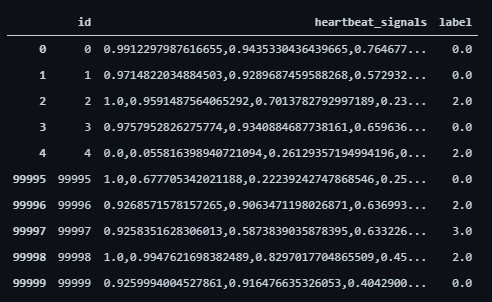
\includegraphics[height=.5\textheight]{image/原数据.jpg}
    \end{figure}
\end{frame}

\section{数据处理}
\begin{frame}
    \frametitle{数据处理}
    \begin{enumerate}
        \item 通过替换数据类型、用category类代替object类的方法来减小内存占用
        \item 将heartbeat\_signals列分割成小的特征
        \item 观察到id列无缺省值无异常值,所以在模型拟合时可以去掉,直接用DataFrame的默认索引代替id值
    \end{enumerate}
    \begin{figure}[h]
        \centering
        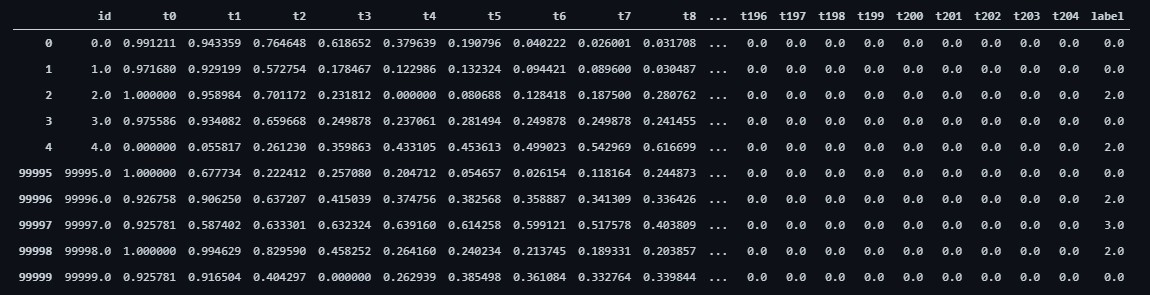
\includegraphics[width=\textwidth]{image/处理后数据.jpg}
    \end{figure}
\end{frame}

\section{方法选用}
\begin{frame}
    \frametitle{方法选用}
    主要考虑到三种方法
    \vspace{1cm}
    \begin{itemize}
        \item AdaBoost
        \item 元分类器是支持向量机(SVM)的AdaBoost
        \item 随机森林 Random Forest
    \end{itemize}
    \vspace{1cm}
    树形结构的算法大多不需要进行降维处理,可以保持特征的可解释性
\end{frame}

\begin{frame}
    \frametitle{AdaBoost}
    \begin{enumerate}
        \item 最常见的AdaBoost元分类器是决策树,sklearn中默认使用一层的决策树来作为它的元分类器
        \item 尝试以不同层数的决策树作为元分类器,精确度先增加后减少
    \end{enumerate}
    \begin{figure}[h]
        \centering
        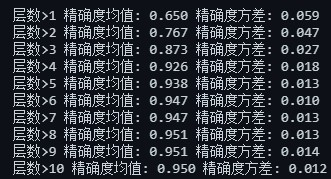
\includegraphics[width=0.5\textwidth]{image/adaboost1.jpg}
    \end{figure}
\end{frame}

\begin{frame}
    \frametitle{AdaBoost + SVM}
    AdaBoost接受所有能样本赋权的分类器作为其元分类器
    \vspace{0.5cm}
    \begin{itemize}
        \item 最常见的赋权分类器有两种,即决策树和支持向量机
        \item 将AdaBoost和SVM结合,尝试找到一个较优的元分类器
        \item 实际效果和一层决策树的AdaBoost一致,并不是很优
    \end{itemize}    
    \begin{figure}[h]
        \centering
        
\includegraphics[width=0.5\textwidth]{image/adaboost2.jpg}
    \end{figure}
    \vspace{0.5cm}
    对比之下,还是决策树更适合与AdaBoost搭配
\end{frame}

\begin{frame}
    \frametitle{Random Forest}
    拟合效果:
\includegraphics[width=0.4\textwidth]{image/randomforest.jpg}
    \begin{block}{随机森林的优势}
    \begin{enumerate}
        \item 随机森林适用于拥有大型数据集的情况,可以处理数千个输入变量而无需变量删除
        \item 能够处理很高维度的数据,并且不用做特征选择(因为特征子集是随机选择的)
        \item 可以在大部分数据丢失时保持准确性
        \item 模型泛化能力强
        \item 对于不平衡的数据集来说,它可以平衡误差
        \item 不需要很多参数调整就可以达到不错的效果
    \end{enumerate}
    \end{block}
\end{frame}

\section{实现}
\begin{frame}
    \frametitle{选取最优方案}
    可以看出以8层决策树为元分类器的AdaBoost和随机森林的准确率较高,表现较好,最终选择使用随机森林
    
    \vspace{0.5cm}
    进一步优化
    \begin{enumerate}
        \item PCA降维,减少随机森林要处理的特征数量,加快随机森林模型的训练速度
        \item 对模型进行超参数调优,进一步提高准确率
    \end{enumerate}
    \vspace{0.5cm}
    计算成本高是随机森林的最大缺点之一,如果只想简单地拥有最佳性能的模型,并且可以牺牲解释特征的重要性,那么PCA可能会很有用,但并不是必须的
\end{frame}

\begin{frame}
    \frametitle{参数调优}
    考虑对模型在未知数据上的评估性能的影响
    \vspace{1cm}
    \begin{enumerate}
        \item 参数n\_estimators的影响最大
        \item max\_depth次之,最大深度也代表了最高复杂度
        \item min\_samples\_leaf和min\_samples\_split并列
        \item max\_features对模型的影响较小
        \item criterion一般使用gini,具体需要视情况而定
    \end{enumerate}
\end{frame}

\begin{frame}
    \frametitle{交叉验证寻找最优n\_estimators}
    先以10为间隔,可以求出在71附近最优
    
    准确率为0.9484999999999999
    \begin{figure}[h]
        \centering
        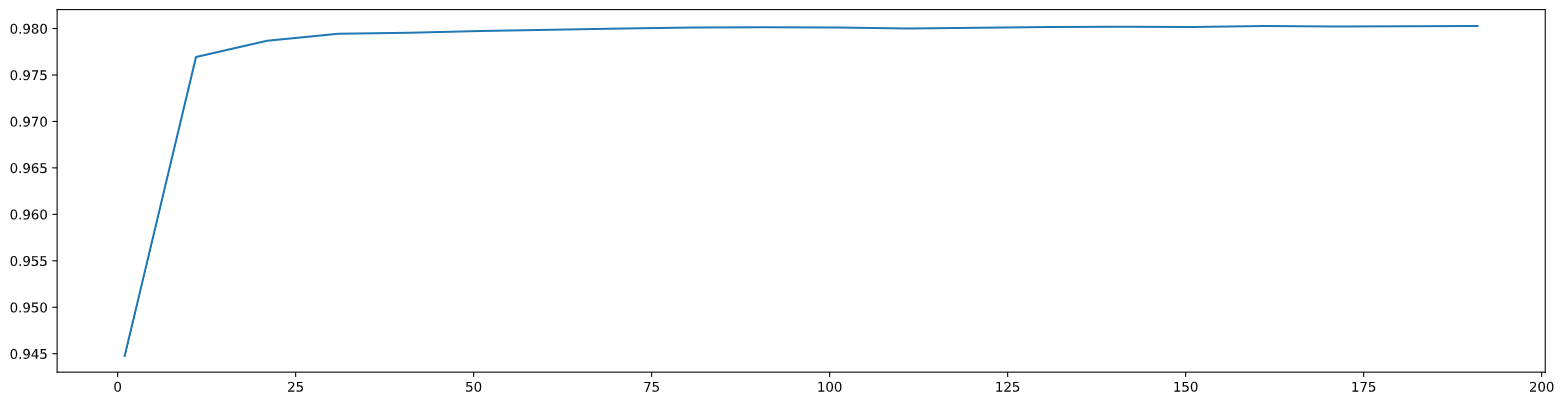
\includegraphics[width=\textwidth]{image/n_estimators.png}
    \end{figure}
\end{frame}

\begin{frame}
    进一步细化,在65-75之间以逐个进行寻找
    
    最终得到最优的n\_estimators为72
    
    此时准确率提高至0.9485000000000001
    \begin{figure}[h]
        \centering
        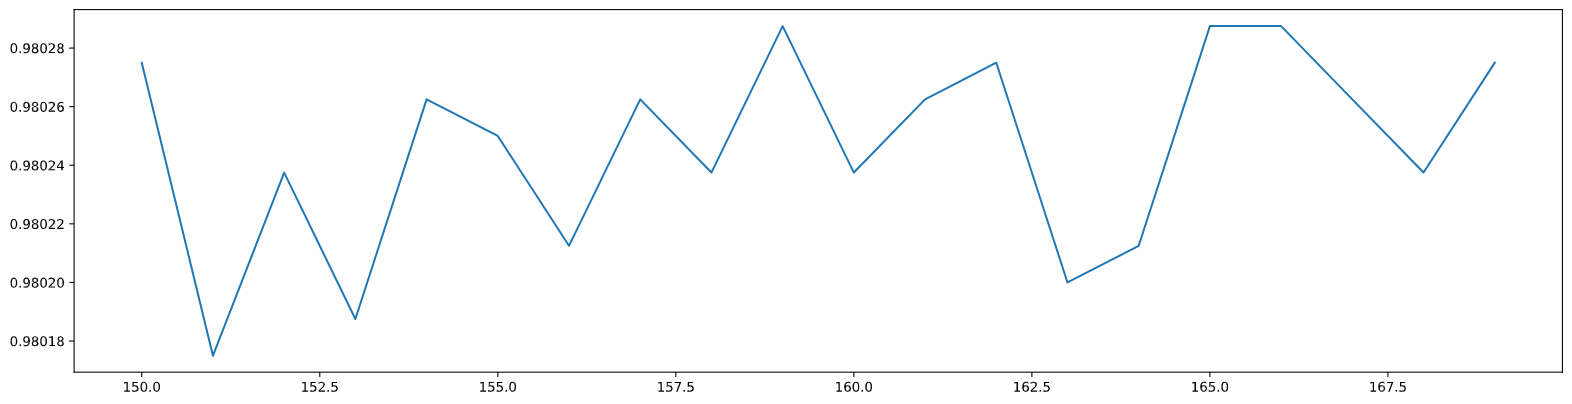
\includegraphics[height=0.5\textheight]{image/n_estimators_final.png}
    \end{figure}
\end{frame}

\begin{frame}
    \frametitle{网格搜索对其余参数进行调优}
    分别对max\_depth min\_samples\_leaf min\_samples\_split max\_features进行网格搜索
    \begin{figure}[h]
        \centering
        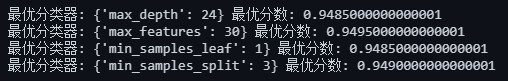
\includegraphics[width=0.9\textwidth]{image/1.jpg}
    \end{figure}
    可以发现原模型已经非常接近模型的上限,max\_features对准确度的提升较大

    最终得到的模型在准确率上提升了0.5\%
    \begin{figure}[h]
        \centering
        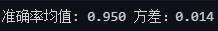
\includegraphics[width=0.4\textwidth]{image/rfc_after_adjust.jpg}
    \end{figure}
\end{frame}

\section{写在最后}
\begin{frame}
    \frametitle{参考内容}
    \begin{enumerate}
        \item \href{https://zhuanlan.zhihu.com/p/44695084}{随机森林 - Random Forest}
        \item \href{https://www.jiqizhixin.com/articles/2020-06-11-6}{决策树VS随机森林}
        \item \href{https://blog.csdn.net/baidu_31657889/article/details/93891552?utm_source=app&app_version=4.7.1}{利用AdaBoost元算法提高分类性能}
        \item \href{https://www.zhihu.com/question/26726794/answer/151282052}{各种机器学习算法的应用场景}
    \end{enumerate}
\end{frame}

\begin{frame}
	\zihao{-4}\centering{Thank you!}
\end{frame}

\end{document}